%Copyright 2019 Christopher M. Jermaine (cmj4@rice.edu) and Risa B. Myers (rbm2@rice.edu)
%
%Licensed under the Apache License, Version 2.0 (the "License");
%you may not use this file except in compliance with the License.
%You may obtain a copy of the License at
%
%    https://www.apache.org/licenses/LICENSE-2.0
%
%Unless required by applicable law or agreed to in writing, software
%distributed under the License is distributed on an "AS IS" BASIS,
%WITHOUT WARRANTIES OR CONDITIONS OF ANY KIND, either express or implied.
%See the License for the specific language governing permissions and
%limitations under the License.
%===============================================================
\documentclass[aspectratio=169]{beamer}
\mode<presentation> 
{
\usetheme[noshadow, minimal,numbers,riceb,nonav]{Rice}
\usefonttheme[onlymath]{serif}
\setbeamercovered{transparent}
}
\useinnertheme{rectangles}

\usepackage[english]{babel}

\usepackage{amsmath}
\usepackage{mathptmx}
\usepackage{helvet}
\usepackage{courier}
\usepackage[T1]{fontenc}
\usepackage{trajan}
\usepackage{ textcomp }
\usepackage{listings}

\newenvironment{noindentitemize}
{ \begin{itemize}
 \setlength{\itemsep}{1.5ex}
  \setlength{\parsep}{0pt}   
  \setlength{\parskip}{0pt}
 \addtolength{\leftskip}{-2em}
 }
{ \end{itemize} }

\newenvironment{noindentitemize2}
{ \begin{itemize}
  \setlength{\itemsep}{0ex}
  \setlength{\parskip}{0pt}
  \setlength{\parsep}{0pt}   
  \addtolength{\leftskip}{-2em}  }
{ \end{itemize} }

\lstnewenvironment{SQL}
  {\lstset{
        aboveskip=5pt,
        belowskip=5pt,
        escapechar=!,
        mathescape=true,
        upquote=true,
        language=SQL,
        basicstyle=\linespread{0.94}\ttfamily\footnotesize,
        morekeywords={WHILE, DO, END},
        deletekeywords={VALUE, PRIOR},
        showstringspaces=true}
        \vspace{0pt}%
        \noindent\minipage{0.47\textwidth}}
  {\endminipage\vspace{0pt}}
  
\newcommand{\LIKES}{\textrm{LIKES}} 
\newcommand{\FREQUENTS}{\textrm{FREQUENTS}} 
\newcommand{\SERVES}{\textrm{SERVES}} 
\newcommand{\CAFE}{\textrm{CAFE}} 
\newcommand{\COFFEE}{\textrm{COFFEE}} 
\newcommand{\DRINKER}{\textrm{DRINKER}} 
\newcommand{\ALLPEEPS}{\textrm{ALLPEEPS}} 
\newcommand{\ALLCOMBOS}{\textrm{ALLCOMBOS}} 


\setbeamerfont{block body}{size=\tiny}

%===============================================================%

\title[]
{Tools \& Models for Data Science}

\subtitle{Sequential Models}

\author[]{Chris Jermaine \& Risa Myers}
\institute
{
  Rice University 
}

\date[]{}

\subject{Beamer}

\begin{document}

\begin{frame}
 \titlepage
\end{frame}
%***********************************************************
\begin{frame}{So Far, Talked About ``iid'' Data}

\begin{itemize}
	\item ``iid'' = independent and identically distributed
	\item Each observation independent
        \item Not always realistic!
	\item Often, data are sequential  (and therefore, not iid)
        \begin{itemize}
		\item Temperature readings
		\item Words in a sentence
		\item Parts of speech: noun followed by verb $\cdots$
		\item Stock prices
		\item Many others!
        \end{itemize}
	\item How can we make predictions in sequences?
	\item How can we solve a labeling problem in sequences?
\end{itemize}
\end{frame}
%***********************************************************
\begin{frame}{``Markov Models''}

\begin{itemize}
	\item Ubiquitous in data science
	\item Basic idea:
	\begin{itemize}
		\item Data observed at a sequence of ``time ticks''
		\item Data at time tick $t$ is $x_t$
		\item \textbf{Markov Assumption}: $x_t$ depends only on $x_{t-1}$
		\item (Or on $x_{t-d}, x_{t-d+1}, x_{t-d+2}, ..., x_{t-1}$ for order-$d$ model)
		\item $d$ is the number of time ticks in the past that contribute to the current time tick
		\item Order $d$ and Order 1 are not all that different
		\item Asset: Going back 5 time ticks is not really more powerful, since the intermediary states can carry forward the information
	\end{itemize}
\end{itemize}
\end{frame}
%***********************************************************
\begin{frame}{Markov Model Order}

\begin{itemize}
		\item $d = 1$\\
		\includegraphics[width=0.8\textwidth]{lectSeq/ar.pdf}
\vspace{1em}
		\item $d = 2$\\
		\includegraphics[width=0.8\textwidth]{lectSeq/ar2.pdf}
\end{itemize}
\end{frame}
%***********************************************************
\begin{frame}{Classic Sequential Model From Stats}

\begin{itemize}
\item The ``Autoregressive'' Model
\item Simple extension of linear regression
	\begin{itemize}
		\item We are doing something like linear regression on the last $d$ observations
		\item Basically, compute the expected value of the next point, using a linear model of the last $d$ points
		\item Order-$d$ model is called an AR($d$) model
	\end{itemize}
	\item As $d$ increases, the plots get smoother
\end{itemize}
% replace these!
%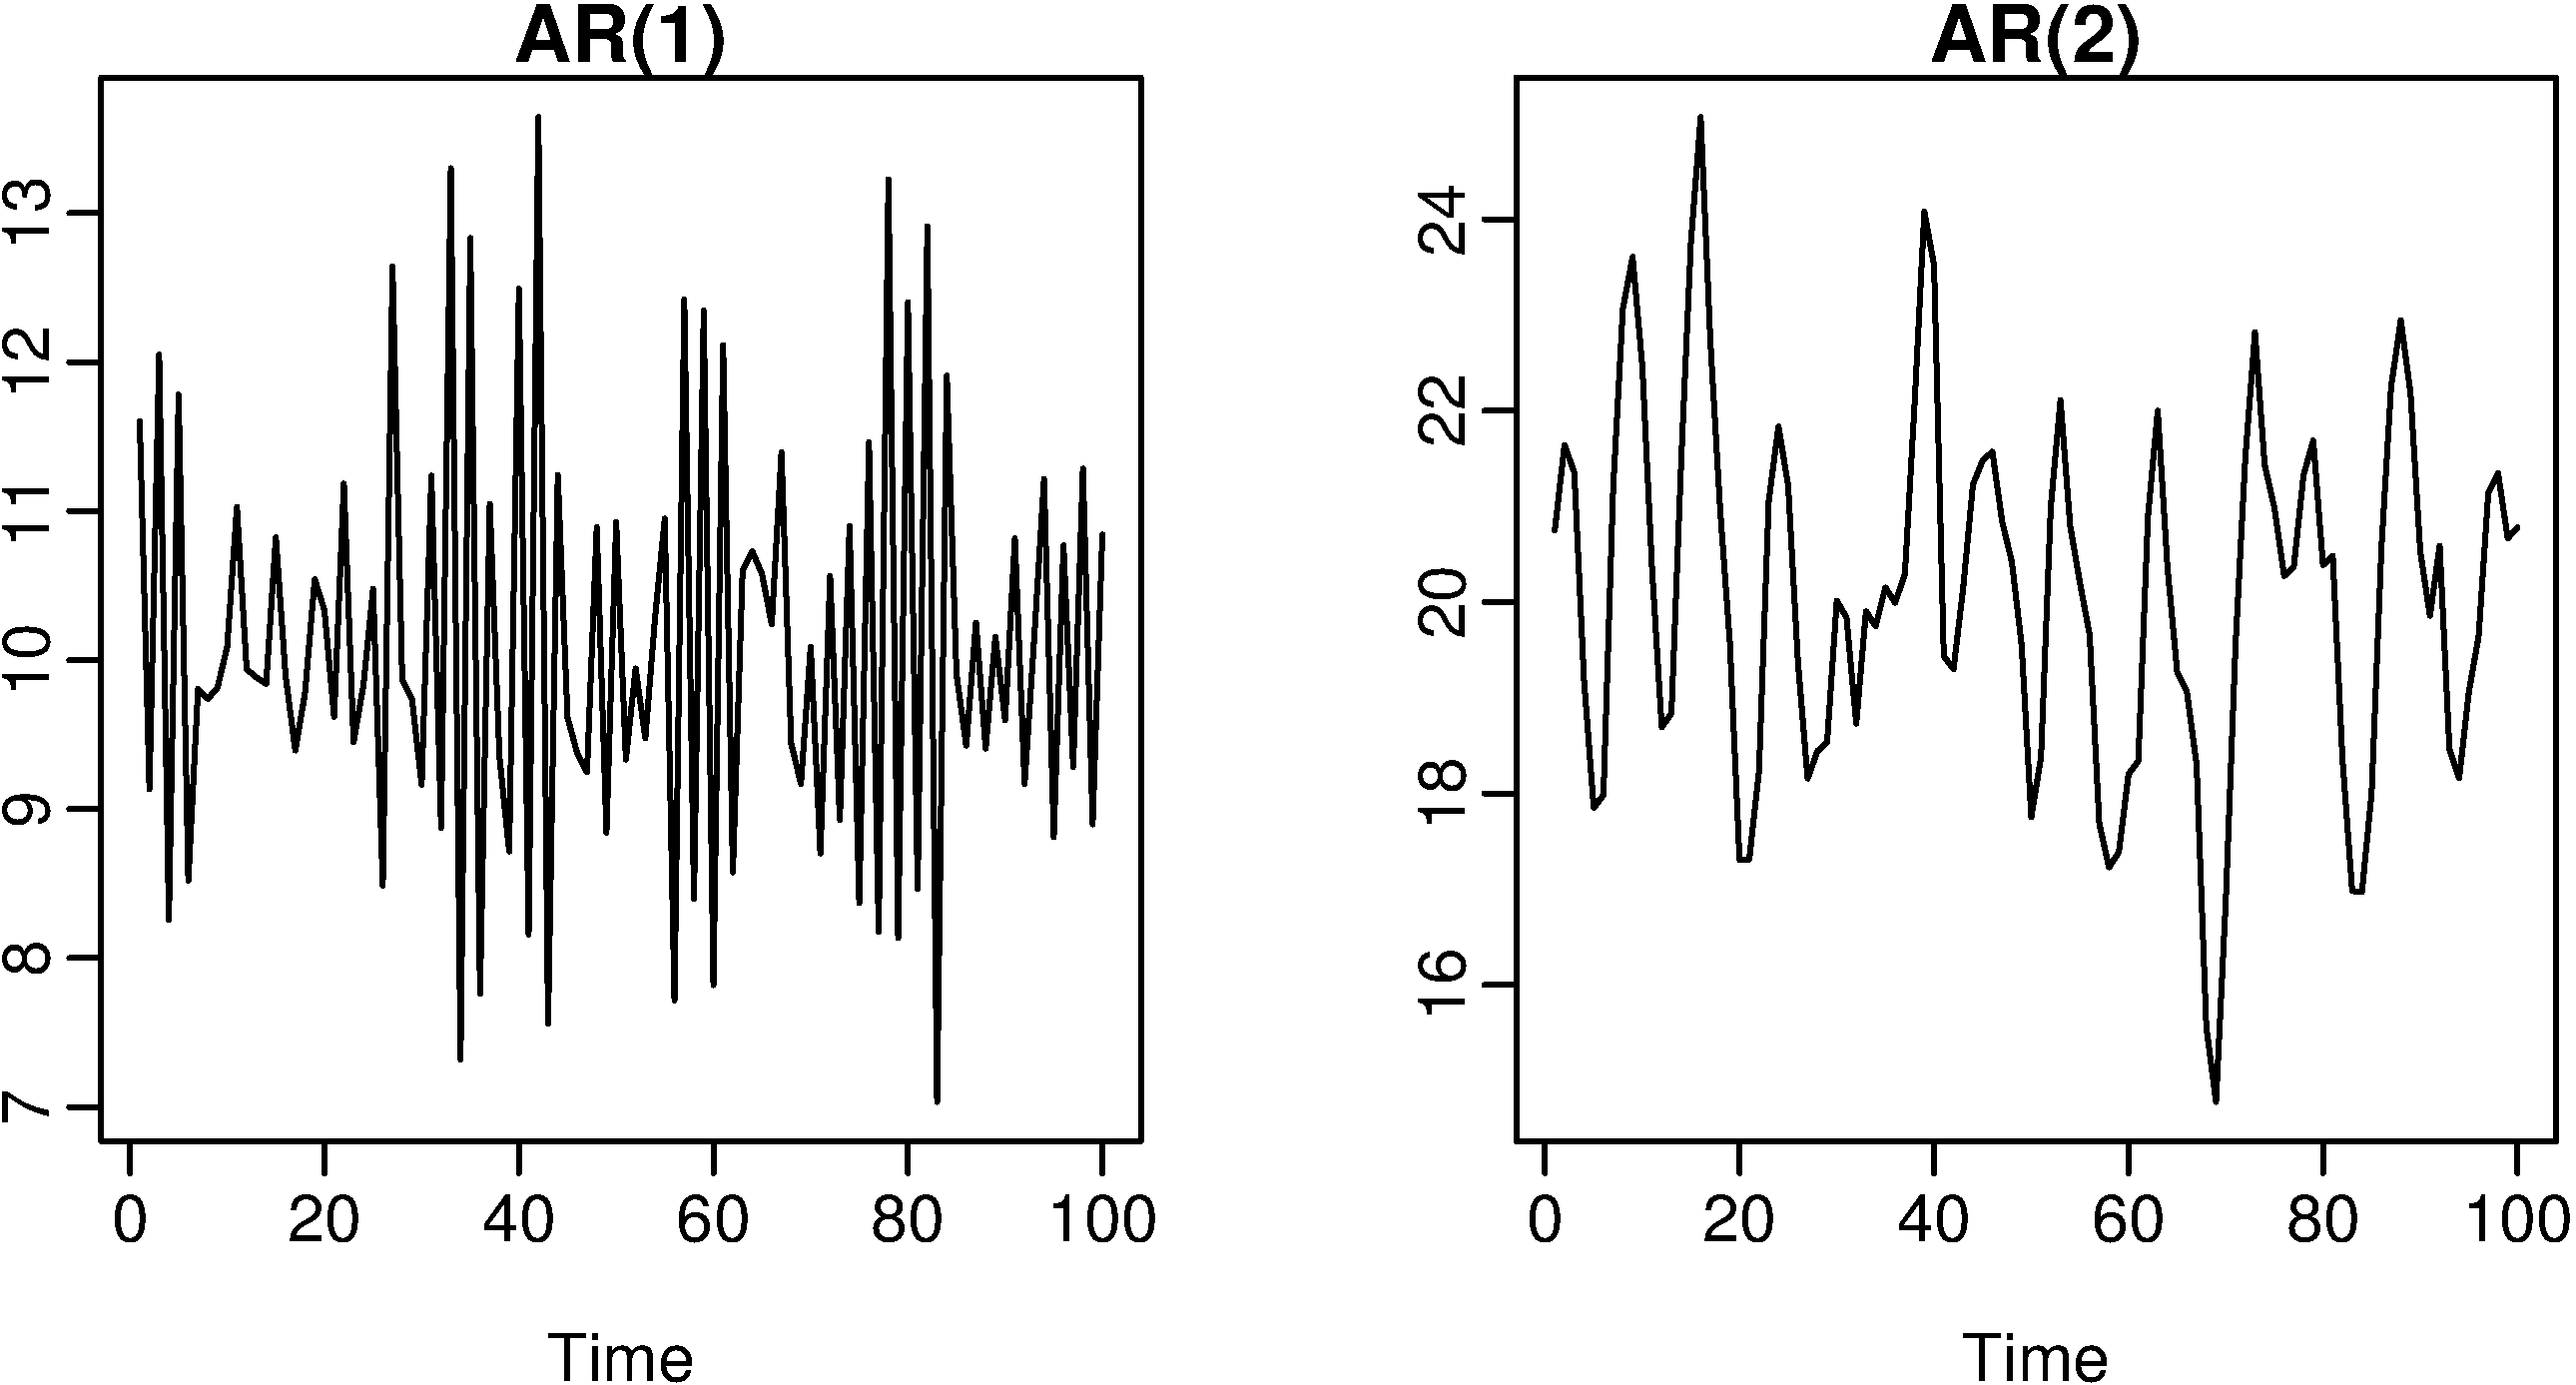
\includegraphics[width=0.5\textwidth]{lectSeq/arp.png}
\end{frame}
%***********************************************************
\begin{frame}[fragile]{Classic Sequential Model From Stats}

\begin{itemize}
\item The ``Autoregressive'' Model
\item Simple extension of linear regression
	\begin{itemize}
		\item Order-$d$ model is called an AR($d$) model
		\item Have $d$ regression coefs for an order-$d$ model
		\item $r_1, r_2, ..., r_d$
	\end{itemize}
\item Generative process is:
\end{itemize}
\begin{columns}
\begin{column}{0.3\textwidth}
\begin{SQL}
1 For $t$ = 1 to $d$ do:
2   $x_t \sim \textrm{Normal}(\mu, \sigma^2)$
3 For $t$ = $d + 1$ to $n$ do:
4  $\theta = \sum_{i = 0}^{d - 1} r_{i + 1} \times x_{t - d + i}$ 
5  $x_t \sim \textrm{Normal}(\theta, \sigma^2)$
\end{SQL}
\end{column}
\begin{column}{0.64\textwidth}
\begin{enumerate}
\item Initialize model  generate first $d$ data points
\vspace{3em}
\addtocounter{enumi}{2}
\item Dot product of regression coefficients with $d$ observations gives the Expected value
\item Sample from a Normal distribution with that mean
\end{enumerate}
\end{column}
\end{columns}

\end{frame}
%***********************************************************
\begin{frame}{Example}

\begin{columns}
\begin{column}{0.4\textwidth}
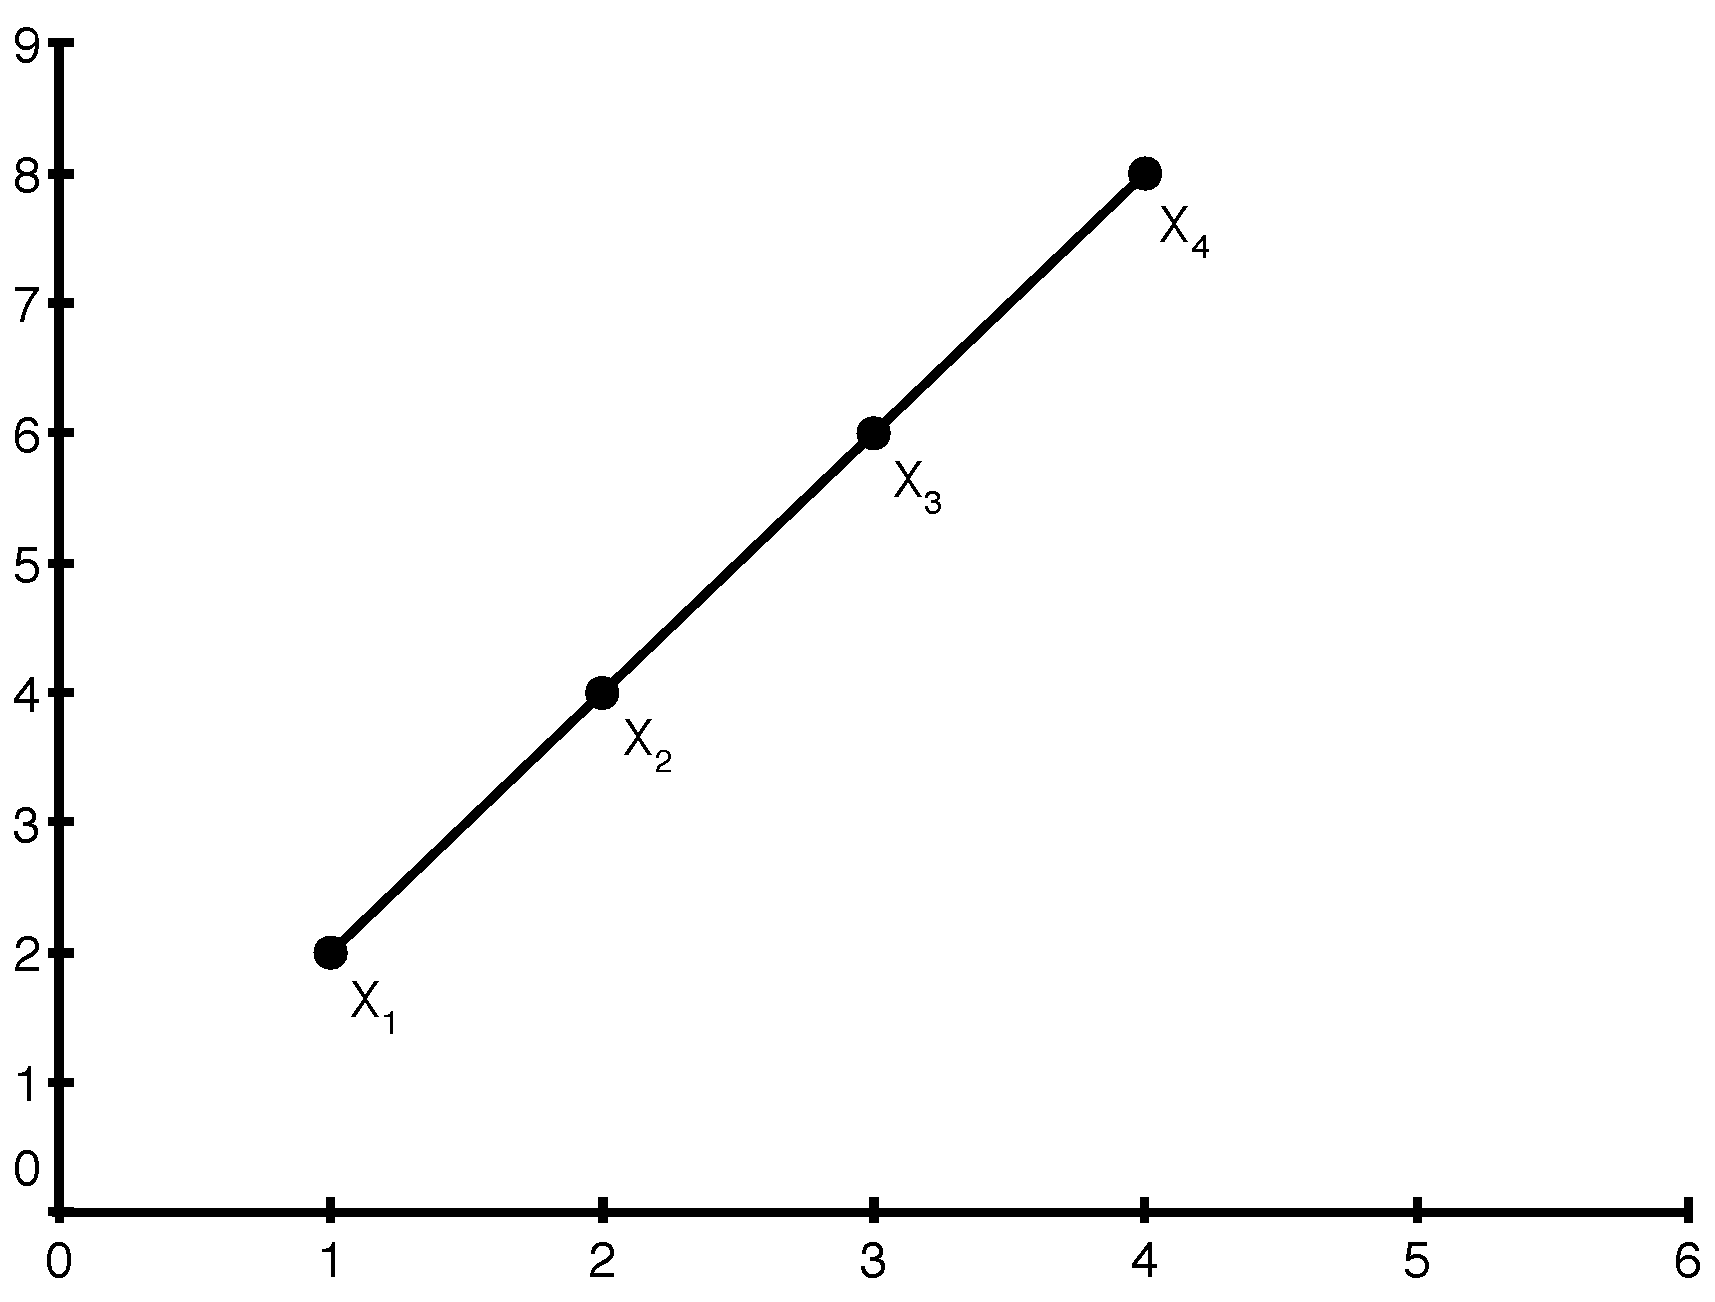
\includegraphics[width=1\textwidth]{lectSeq/ARLR.pdf}
\end{column}
\begin{column}{0.6\textwidth}
\begin{itemize}
\item To continue the trajectory, we need at least AR(2)
\item Assume the step same step size to X$_4$ as was to X$_3$
\item Assume each time tick is uniform
\item Here, r = $<2, -1>$
$$x_n = r_0 x_{n-1} + r_1 x_{n-2}$$
\end{itemize}
\end{column}
\end{columns}
\end{frame}
%***********************************************************
\begin{frame}{Definitions \& Properties}

\begin{itemize}
\item Markov Property
\begin{itemize}
\item Future state depends only on the current state
\end{itemize}
\item Markov Chain
\begin{itemize}
\item Stochastic process with the Markov Property
\item May have an infinite number of states
\end{itemize}
\item Markov Process
\begin{itemize}
\item Stochastic process that transitions between states using provided probabilities
\end{itemize}
\item Markov Model
\begin{itemize}
\item Commonly viewed as any sequential model with a finite dependency back in time
\item Really means a finite state Markov Chain
\end{itemize}
\end{itemize}
\end{frame}
%***********************************************************
\begin{frame}{Classic Sequential Model from CS}

\begin{itemize}
\item Markov Model
	\begin{itemize}
	\item Begins with a Markov chain
	\item Assume that there are $m$ states
	\item We stochastically jump around between the states
	\end{itemize}
\end{itemize}
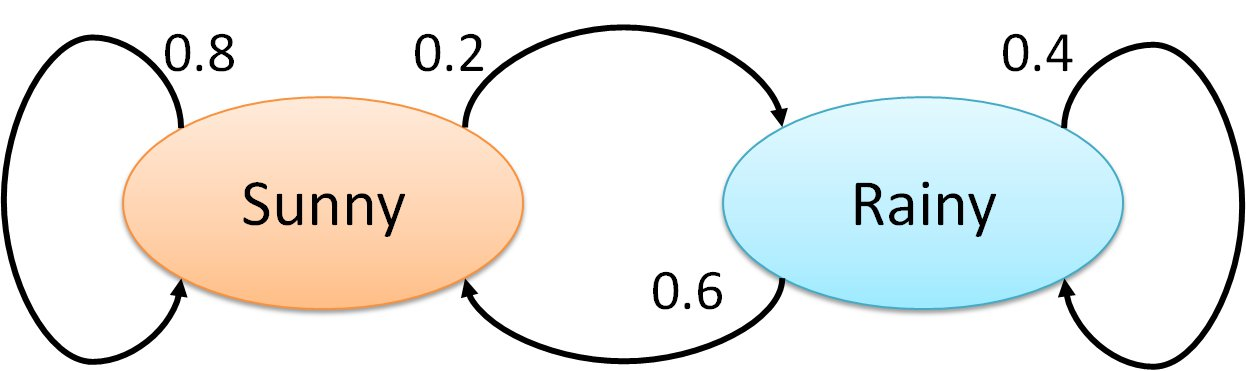
\includegraphics[width=0.8\textwidth]{lectSeq/markov-chain1.jpg}
\end{frame}
%***********************************************************
\begin{frame}[fragile]{Classic Sequential Model from CS}

\begin{itemize}
\item Markov Model
	\begin{itemize}
	\item Begins with a Markov chain
	\item Assume that there are $m$ states
	\item We stochastically jump around between the states
	\item Let $\pi_0$ be  start probabilities
	\item Let $\pi_i$ be transition probabilities out of state $i$
	\item Let $s_1$ be the start state selected from the start probabilities
	\end{itemize}
\end{itemize}
\begin{SQL}
$s_1 \sim \textrm{Categorical}(\pi_0)$
For $t$ = 2 to $n$ do:
  $s_t \sim \textrm{Categorical}(\pi_{s_{t - 1}})$
\end{SQL}

\end{frame}
%***********************************************************
\begin{frame}{Categorical Distribution}

\begin{itemize}
	\item Bernoulli distribution generalized for more than 2 choices
	\item Outcomes are discrete
	\item Each outcome has a probability
	\item Probabilities sum to 1
	\item Example
		\begin{itemize}
			\item 10 balls into 5 baskets
			\item Multinomial distribution tells you how the balls are distributed within the baskets
			\item Categorical distribution tells you will basket a single ball landed in
		\end{itemize}
	\item Another Example
		\begin{itemize}
			\item Throw a weighted die
			\item The side facing up is the selected category
		\end{itemize}
\end{itemize}

\end{frame}
%***********************************************************
\begin{frame}{HMM}

\begin{itemize}
\item Hidden Markov Model
\item Called ``hidden'' because we typically don't observe states
\item We just see emitted values
\item Most common type of Markov model
\end{itemize}
\end{frame}
%***********************************************************
\begin{frame}[fragile]{HMM}

\begin{itemize}
\item Then we add the observed data
	\begin{itemize}
	\item Often Categorical
	\item Though sometimes not (Normal, Gamma, Poisson are common)
	\item Let $\theta_s$ be parameter set associated with state $s$
	\end{itemize}
\item Called ``hidden'' because we typically don't observe states
\end{itemize}
\begin{columns}
\begin{column}{0.4\textwidth}
\begin{SQL}
$s_1 \sim \textrm{Categorical}(\pi_0)$
$x_1 \sim f(\theta_{s_1})$
For $t$ = 2 to $n$ do:
  $s_t \sim \textrm{Categorical}(\pi_{s_{t - 1}})$
  $x_t \sim f(\theta_{s_{t}})$
\end{SQL}
\end{column}
\begin{column}{0.6\textwidth}
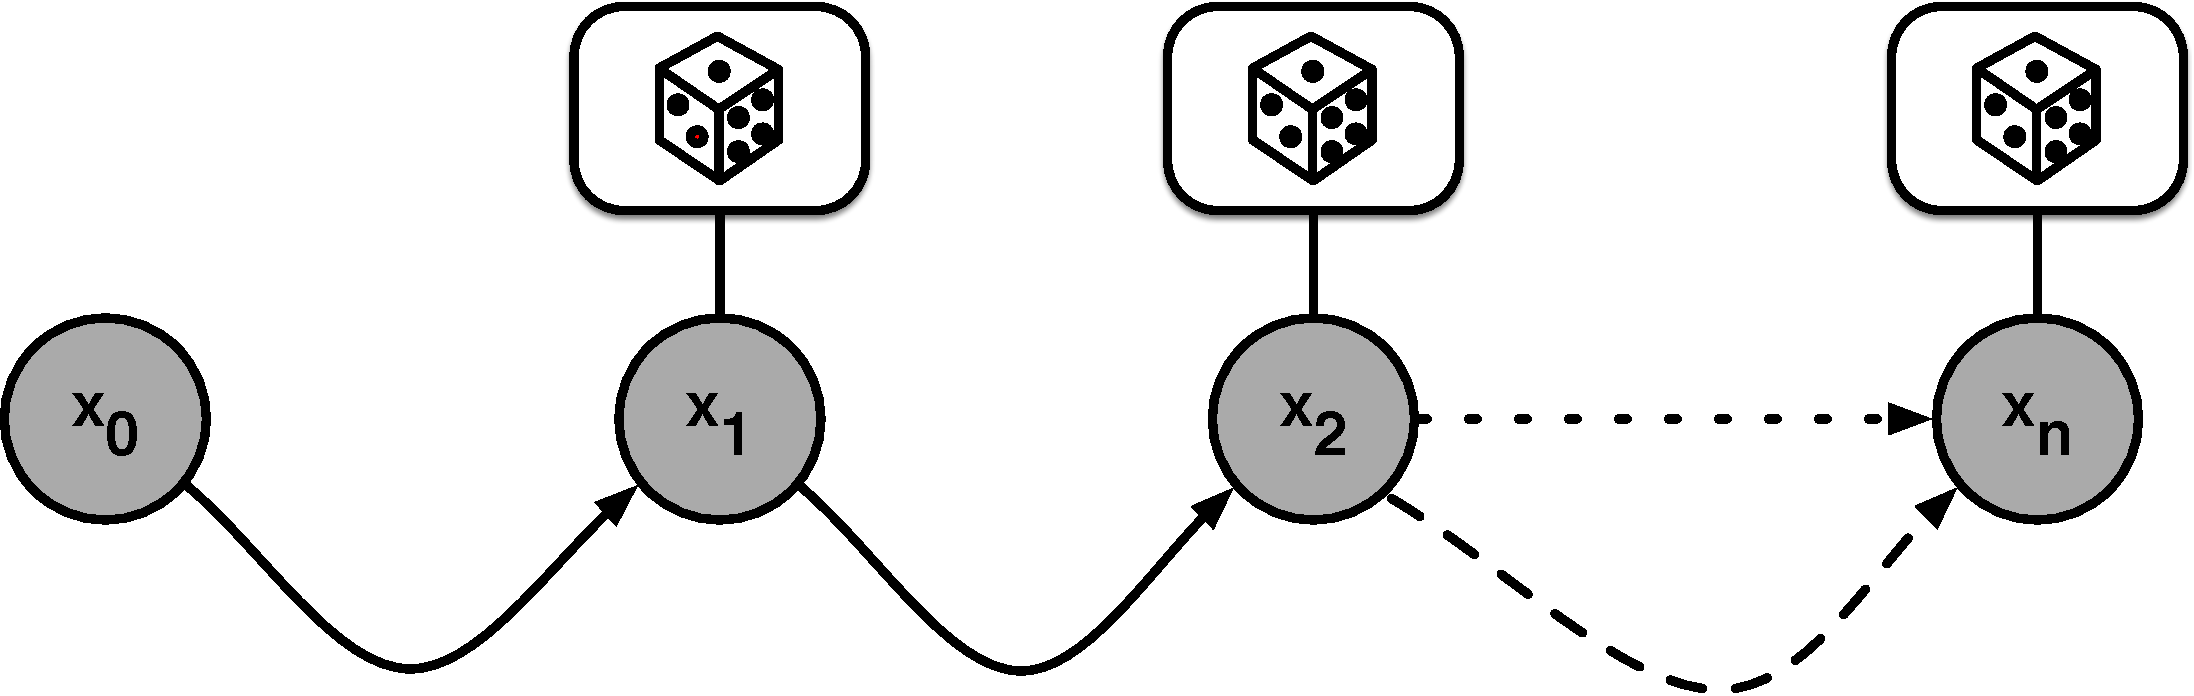
\includegraphics[width=1\textwidth]{lectSeq/autoregressiveCat.pdf}
\end{column}
\end{columns}

\end{frame}
%***********************************************************
\begin{frame}{Example HMM}

\begin{columns}
\begin{column}{0.6\textwidth}
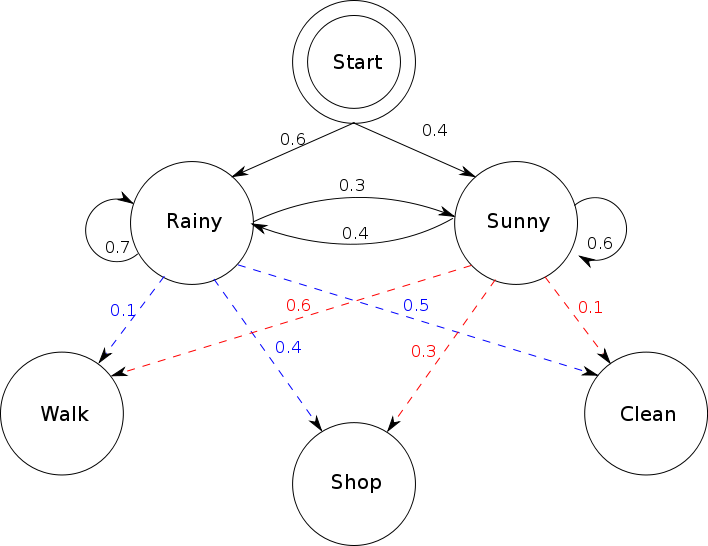
\includegraphics[width=1\textwidth]{lectSeq/708px-HMMGraph.png}
\end{column}
\begin{column}{0.4\textwidth}
\begin{itemize}
\item $\pi_0 = [ 0.6\ \ 0.4]$
\item $\pi$ matrix 
\begin{equation}
  \begin{bmatrix}
  0.7 & 0.3 \\\nonumber
  0.4 & 0.6  \\ 
  \end{bmatrix}
\end{equation}
\item Categorical output. Different probabilities based on current state
\end{itemize}
\end{column}
\end{columns}
\end{frame}
%***********************************************************

\begin{frame}{Making Predictions using an HMM}

\begin{itemize}
\item Problem: Predict the observation at $x_{n+1}$
\item Given an HMM
\item and a sequence $S = \langle x_1, x_2, ..., x_n \rangle$
\item How to do it? 
\end{itemize}

\end{frame}
%***********************************************************

\begin{frame}{Making Predictions using an HMM}

\begin{itemize}
\item Problem: Predict the observation at $x_{n+1}$

\item  Basic idea:
	\begin{itemize}
	\item First, for each state $s$, find $p^{(n)}_s$
	\item This is probability of being in state $s$ at time tick $n$
	\item Then, compute $p^{(n+1)}_s = \sum_{s'} p^{(n)}_{s'} \pi_{s',s}$
	\item $\pi_{s',s}$ is probability of transitioning from state $s'$ from $s$
	\item Since we sum over all ways to get to $s$ from tick $t$, $p^{(n+1)}_s$ is probability of state $s$ at tick $n+1$
	\item And choose $x_{n+1} = \textrm{argmax}_{x_{n+1}} \sum_s p^{(n+1)}_s f(x_{n+1} | \theta_{s})$
%	\item (integrate over all possible states at tick $n$ and determine the probability of getting to the new state and getting the new observation)
	\item Now we have our prediction!
	\end{itemize}
\item BUT, still need to find $p^{(n)}_s$ for each $s$. How?
\end{itemize}

\end{frame}
%***********************************************************

\begin{frame}{Making Predictions using an HMM}

\begin{itemize}
\item Problem: Predict the observation at $x_{n+1}$

\item In other words:
	\begin{itemize}
	\item Figure out the most likely combination of where you are 
	\item ... and where you are going 
	\item Based on where you know you are, the transition probabilities, and the emission probabilities
	\end{itemize}	
\item For example
	\begin{itemize}
	\item If you stayed home and cleaned, what are you likely to do tomorrow?
	\end{itemize}	

\item BUT, still need to find $p^{(n)}_s$ for each $s$. How?
\end{itemize}

\end{frame}
%***********************************************************
\begin{frame}{Finding a Path Thru an HMM}

\begin{itemize}
\item Problem: Predict the observation at $x_{n+1}$
\item How to compute the (posterior) probability we were in state $s$ at each time tick?
\item To do this, let $A[i,j]$ denote
	\begin{itemize}
	\item Probability of us having $s_i = j$
	\item Given that we have observed $\langle x_1, x_2, ..., x_i \rangle$
	\end{itemize}
\item Fill out $A$ using dynamic programming
\end{itemize}
\end{frame}
%***********************************************************
\begin{frame}{What is Dynamic Programming?}

\begin{itemize}
\item Approach to solving problems with overlapping sub-problems
\item The optimal solution must use the optimal sub-problem
\item Basically, save your solutions 
\item Solve the base case
\item Solve the recursive relationship
\item Example: Tower of Hanoi
\item Contrast with ``divide and conquer''
	\begin{itemize}
	\item Break a problem with  non-overlappying sub-problems into pieces
	\item Solve the sub-problems
	\item Combine results
	\end{itemize}
\end{itemize}
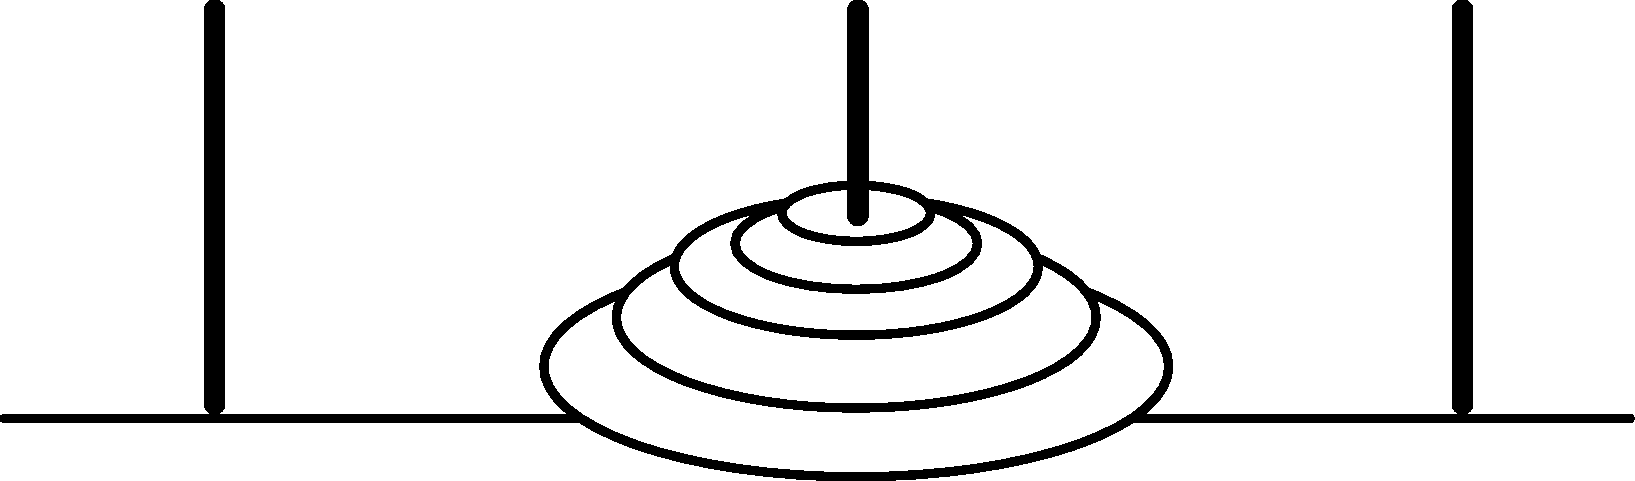
\includegraphics[width=.5\textwidth]{lectSeq/hanoi.pdf}
\end{frame}
%***********************************************************
\begin{frame}{Common Application of  Dynamic Programming?}
\begin{columns}[T]
\begin{column}{0.5\textwidth}
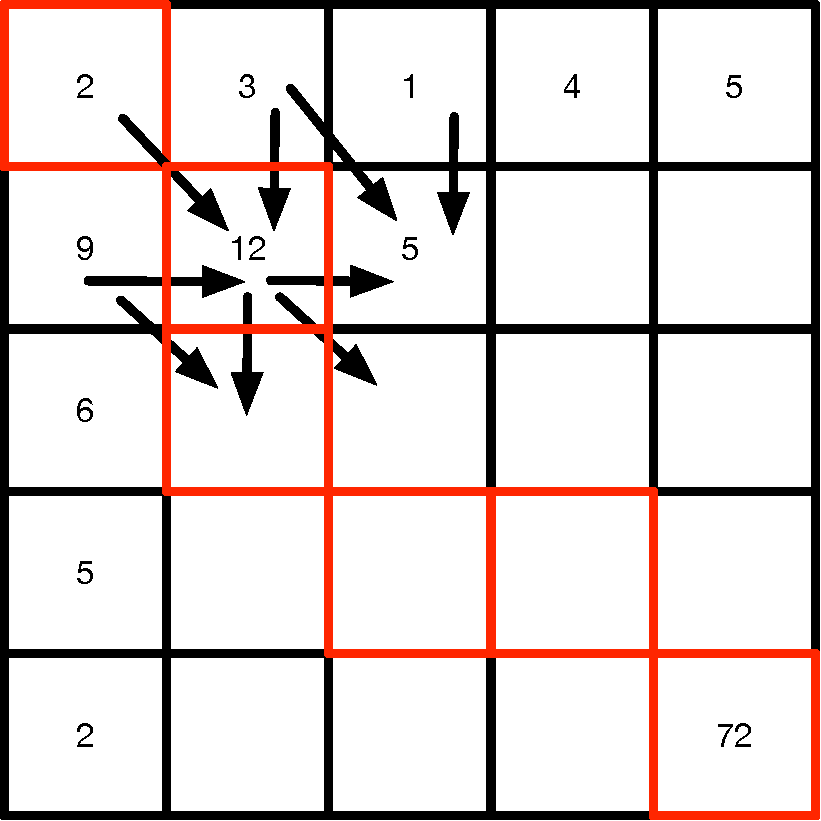
\includegraphics[width=1\textwidth]{lectSeq/dp.pdf}
\end{column}
\begin{column}{0.5\textwidth}
	\begin{itemize}
	\item Populate top row and left column via base cases
	\item Populate internal cells from rule based on neighbors above and to the left
	\item Begin in upper left
	\item End in lower right
	\end{itemize}
\end{column}
\end{columns}
\end{frame}

%***********************************************************

\begin{frame}{How to Compute the DP Matrix?}

\begin{columns}[T]
\begin{column}{0.5\textwidth}
\begin{itemize}
\item Base case:
	\begin{itemize}
	\item $A[1,j] \propto \pi_{0,j} \times f (x_1 | \theta_j)$
	\item Then normalize so $A[1,j] = \frac{A[1,j]}{\sum_{j'} A[1,j']}$
	\item Note, normalization comes out of Bayes' rule: Pr[$s_1 = j$ given $x_1$] is...
	\item Pr[$s_1 = j$ and $x_1$] / Pr[$x_1$]
	\end{itemize}
\end{itemize}
\end{column}
\begin{column}{0.5\textwidth}
	\begin{itemize}
	\item $\pi_{0,j}$ = Probability of being in state $j$ at tick 1
	\item $f (x_1 | \theta_j) = $ LLH of emitting $x_1$
	\end{itemize}
\end{column}
\end{columns}
\end{frame}
%***********************************************************

\begin{frame}{How to Compute the DP Matrix?}

\begin{columns}[T]
\begin{column}{0.5\textwidth}
\begin{itemize}
\item Recurrence:
	\begin{itemize}
	\item $A[i,j] \propto \sum_{j'} A[i-1,j'] \times \pi_{j',j} \times f (x_1 | \theta_j)$
	\item Then normalize so $A[i,j] = \frac{A[i,j]}{\sum_{j'} A[i,j']}$
	\item Note, normalization again comes out of Bayes' rule
	\end{itemize}
\item Now we can do our prediction!
\item Use DP to compute $A$ matrix
\item Then use $p^{(n)}_s = A[n,s]$ to make prediction
\end{itemize}
\end{column}
\begin{column}{0.5\textwidth}
	\begin{itemize}
	\item $A[i,j] = $ Pr( in state $j$ at tick $i$ | $x_1, x_2, \cdots, x_n$) 
	\item $A[i-1,j']$ = Pr( I was in the last state) 
	\item multiply $A[i-1,j']$ by 
	\item $\pi_{j',j}$ the transition probability
	\item and $f (x_1 | \theta_j)$ the emission probability
	\end{itemize}
\end{column}
\end{columns}
\end{frame}
%***********************************************************

\begin{frame}{Now We Know How To Compute the Probability of a State}

\begin{itemize}
\item Similar methods can be used to learn an HMM
\item What do we mean by ``learn an HMM''?
\item Given a number of states, $m$
\item And a set of sequential observations $\langle x_1, x_2, ..., x_n \rangle$
\item Learn 
\begin{itemize}
\item $\pi_0$, the start probabilities
\item $\pi$, the transition probabilities between states
\item The parameters, $\theta_s$ of the emission distribution for each state $s$ 
\end{itemize}
\end{itemize}
\end{frame}
%***********************************************************

\begin{frame}{Now We Know How To Compute the Probability of a State}

\begin{itemize}
\item Similar methods can be used to learn an HMM
\item Relies on an EM algorithm
\item Why EM?
\begin{itemize}
\item Missing data: we don't know the state at each time tick
\item EM is meant to solve MLE given missing data
\item EM for HMM aka ``Baum-Welch algorithm''
\end{itemize}
\item We won't derive the EM algorithm from the EM $Q$ function
\item We begin with the E-step
\begin{itemize}
\item We need to be able to compute the probability that we are in state $j$ at tick $i$, given a model
\item DP algorithm to do this is often called ``forward-backward algorithm''
\end{itemize}
\end{itemize}
\end{frame}
%***********************************************************

\begin{frame}{EM For Learning a HMM}

\begin{itemize}
\item Let $C[i,j]$ be the probability that we are in state $j$ at tick $i$
	\begin{itemize}
	\item Given ALL of $\langle x_1, x_2, ..., x_n \rangle$
	\end{itemize}
\item How to compute?  DP! Two other matrices will help...
\item This is where the name comes from
\item Forward: Let $\alpha[i,j]$ denote the probability
	\begin{itemize}
	\item Of observing $\langle x_1, x_2, ..., x_i \rangle$
	\item AND ending in state $j$
	\item Takes into account everything before this time tick
	\end{itemize}
\item Backward: Let $\beta[i,j]$ denote the probability
	\begin{itemize}
	\item Of observing $\langle x_{i+1}, ..., x_n \rangle$
	\item Given we start in state $j$
	\item takes into account everything after this time tick
	\end{itemize}
\item We combine these matrices to compute C
\end{itemize}
\end{frame}
%***********************************************************
\begin{frame}{Combining the Two Probabilities}

\begin{itemize}
\item Why do these help?
\item Note that $C[i,j]$ is probability we are in state $j$
	\begin{itemize}
	\item Given $\langle x_1, x_2, ..., x_i \rangle$
	\item AND given $\langle x_{i+1}, x_2, ..., x_n \rangle$
	\end{itemize}
\item From Bayes' rule
\item[] \text{Pr[in state } j  | \text{sequence until } i\text{, sequence after }i\text{]} = $C[i,j] = \frac{\text{Pr[in state } j \text{ with sequence until } i \text{ and sequence after } i\text{]} }{\text{Pr[whole sequence]}}$
%	\begin{itemize}
%	\item $C[i,j] = $ Pr[in state $j$ | sequence until $i$, sequence after $i$]
%	\item is Pr[in state $j$ with sequence until $i$ and sequence after $i$] divided by
%	\item Pr[whole sequence]
%	\end{itemize}
\item So $C$ can be expressed in terms of $\alpha$ and $\beta$
	 $$C[i,j] = \frac{\alpha[i,j] \beta[i,j]}{\sum_{j'} \alpha[i,j'] \beta[i,j']}$$

\item Still need to compute $\alpha$, $\beta$
\end{itemize}
\end{frame}
%***********************************************************

\begin{frame}{The Forward Pass}

\begin{itemize}
\item Recall $\alpha[i,j]$ denotes the probability
	\begin{itemize}
	\item Of observing $\langle x_1, x_2, ..., x_i \rangle$
	\item AND ending in state $j$
	\end{itemize}
\item Compute with DP! Base case: probability of being in state $j$ and observing the first output
        \begin{itemize}
        \item $\alpha[1,j] \propto \pi_{0,j} \times f(x_1 | \theta_j)$
        \item Recall: $\pi_0$ is the vector of start probabilities
        \item $f(x_1 | \theta_j)$ is the probability of emitting $x_1$
        \end{itemize}
\item Recurrence
	\begin{itemize}
	\item $\alpha[i,j] \propto f(x_i | \theta_j) \times \sum_{j'}\Big( \pi_{j',j} \times \alpha[i-1,j']\Big)$ 
	\item entry $\propto$ LLH of observation from state $j \times$ sum over all possible ways to get to state $j$
	\end{itemize}
\end{itemize}
\end{frame}
%***********************************************************

\begin{frame}{The Backward Pass}

\begin{itemize}
\item Recall $\beta[i,j]$ denotes the likelihood
	\begin{itemize}
	\item Of observing $\langle x_{i+1}, ..., x_n \rangle$
	\item Given we start in state $j$
	\end{itemize}
\item Again, compute with DP! Base case
        \begin{itemize}
        \item $\beta[n,j] = 1$
        \item We want the probability I see everything in the future if I'm in state $j$
        \item But, I'm at tick $n$, so there is no future
        \item The probability I observe nothing when I'm done is 1
        \end{itemize}
\item Recurrence
	\begin{itemize}
	\item $\beta[i,j] \propto \sum_{j'} \Big( \pi_{j,j'} \times f(x_{i+1} | \theta_{j'}) \times \beta[i+1,j'] \Big)$ 
	\item The recursion happens backwards
	\item Start in state $j$ 
	\item Consider all possible next states in the next time tick, taking into account $\pi_{j,j'}$
	\item $\beta[i+1, j']$ = how well does $j'$ explain everything in the future $(i+2, i+3, \cdots)$
%	\item entry $\propto $ one step in the future
	\end{itemize}
\end{itemize}\end{frame}
%***********************************************************

\begin{frame}{That's The E-Step!}

\begin{itemize}
\item Let's relate this back to the coin flip EM
\begin{itemize}
\item[?] E-step: What was missing? 
\end{itemize}
\end{itemize}
\end{frame}
%***********************************************************

\begin{frame}{That's The E-Step!}

\begin{itemize}
\item Let's relate this back to the coin flip EM
\begin{itemize}
\item E-step: What was missing? 
\item The identity of the coin
\item We computed the probability of the coin identity each time we reached into the bag
\item Given the current parameters, what's the probability that the current coin is coin 1? coin 2?
\item Say we see HHHTHH
\item and we estimate the probability of HEADS for the coins as $\langle 0.8, .03 \rangle$
\item[?] Which coin was more likely to generate that sequence?
\vspace {1em} 
\item $C[i,j]$ gives us the probability I'm in state $j$ given the entire sequence
\end{itemize}
\item How about the M-Step?
\end{itemize}
\end{frame}
%***********************************************************

\begin{frame}{First: Estimate the Distributional Params}

\begin{itemize}
\item Need to update each parameter $\theta_j$
	\begin{itemize}
	\item Set each $\theta_j$ to 
	\begin{align}
		\textrm{argmax}_{\theta_j} \sum_i \log C[i,j] f(x_i | \theta_j) \nonumber
	\end{align}
	\item Note: If $C[i,j]$ is large, then that observation is more tightly coupled with that state
	\end{itemize}
\item What's going on here?
	\begin{itemize}
	\item We are doing a MLE
	% Take partial derivatives, etc. of the argmax
	\item Weighted on $C[i,j]$
	\item Which is the probability that we were in state $j$ at time $i$
	\item Given the current model
	\end{itemize}
\end{itemize}
\end{frame}
%***********************************************************

\begin{frame}{Estimating the Transition Probs}

\begin{itemize}
\item Consider D[2, sunny, rainy] = certainty I was in the sunny state at tick 2 and rainy state at tick 3
\item Define $D[i,j,k]$ to be
	\begin{itemize}
	\item The probability of being in state $j$ at time $i$
	\item AND being in state $k$ at time $i+1$
	\item AND seeing the entire sequence
	\item Can be computed as
	$$\frac{\alpha[i,j] \pi_{j,k} \beta[i+1,k] f(x_{i+1} | \theta_k)}
	{\sum_{j',k'} \alpha[i,j'] \pi_{j',k'} \beta[i+1,k'] f(x_{i+1} | \theta_{k'})}$$
	\end{itemize}
	\item Why? Recall: $\alpha[i,j]$ is probability of $\langle x_1, ..., x_i \rangle$ and ending in state $j$
	\item $\beta[i+1,k]$ is probability of $\langle x_{i + 2}, ..., x_n \rangle$ starting in state $k$
	\item $\pi_{j,k}$ is prob of transition from state $j$ to state $k$
	\item $f(x_{i+1} | \theta_k)$ is probability of emitting $x_{i+1}$ in state $k$
	\item Put them together and normalize... exactly the probability we want!
\end{itemize}
\end{frame}

%***********************************************************

\begin{frame}{More about the D Matrix}

	$$\frac{\alpha[i,j] \pi_{j,k} \beta[i+1,k] f(x_{i+1} | \theta_k)}
	{\sum_{j',k'} \alpha[i,j'] \pi_{j',k'} \beta[i+1,k'] f(x_{i+1} | \theta_{k'})}$$
\begin{itemize}
%\item C is about 1 state at time tick $i$
\item D is about both states: state $j$ at tick $i$ and state $k$ at tick $i+1$
\item How does $\pi$ relate to D?
\item $\pi$ is a model parameter, we read it off the state transition diagram
\item It DOESN'T describe a particular run, but rather the expected results
\item D comes from estimating the parameters based on the emissions seen
\item D says how certain I am that I was in the sunny state instead of the rainy state
\end{itemize}
\end{frame}


%***********************************************************

\begin{frame}{Estimating the Transition Probs}

\begin{itemize}
\item Then $\pi_{j,k}$  is estimated as:
	$$\pi_{j,k} = \frac{\sum_i D[i,j,k]} {\sum_i C[i,j]}$$
\item What's going on here?
	\begin{itemize}
	\item $D[i,j,k]$ is the probability that we transitioned from $j$ to $k$ at tick $i$
	\item So we are setting $\pi_{j,k}$ to be fraction of time we transitioned from $j$ to $k$
	\item Out of the total time that we were in $j$
	\end{itemize}
\item And start probs:
	$$\pi_{0,j} = C[1,j]$$
	\begin{itemize}
	\item This is simply the probability that we were in $j$ at tick 0
	\end{itemize}
\end{itemize}
\end{frame}
%***********************************************************

\begin{frame}{Review of EM Steps}

\begin{itemize}
\item Compute $\alpha$ and $\beta$ to get $C$
\begin{itemize}
\item The probability we are in state $j$ at time $i$
\end{itemize}

\item Use $C$ to get $D$
\begin{itemize}
\item The probability we are in state $j$ at time $i$ AND in state $k$ at time $i+1$
\end{itemize}
\item Use these to get $f, \theta$
\begin{itemize}
\item The parameters of the emission function
\end{itemize}
\item Estimate $\pi$ from these
 \begin{itemize}
\item The transition probabilities from state to state
\end{itemize}
\end{itemize}
\end{frame}

%***********************************************************

\begin{frame}{This Allow Us to Learn HMM for One Big Sequence}

\begin{itemize}
\item How to handle many sequences?
\begin{itemize}
\item Have a special symbol $\epsilon$ at the end of each sequence
\item Have a special state $e$ (for ``end'')
\item Set $f(\epsilon|\theta_e) = 1$, $f(x \neq \epsilon|\theta_e) = 0$,  $f(\epsilon|\theta_{s\neq e}) = 0$
\item And just concatenate all of the sequences, learn as a single sequence
\end{itemize}
\item Example: A large number of sentences
\item The emissions are wordso
\item Use an extra state that you transition to every time you get a new sequence / sentence
\end{itemize}
\end{frame}
%***********************************************************

\begin{frame}{Advantages, Disadvantages and Other Algorithms}

\begin{itemize}
\item HMMs are interpretable
\item Recurrent Neural Networks can have higher accuracy
\vspace{1em}
\item Viterbi Algorithm
\begin{itemize}
\item Computes the most likely sequence of hidden states given the emissions
\end{itemize}
\item Dynamic Time Warping
\end{itemize}
\end{frame}

%***********************************************************

\begin{frame}{Dynamic Time Warping}

\begin{itemize}
\item Pairwise comparison of time series for classification
\item Allows for distortion in the time dimension
\item Works well for pattern matching
\item Used in conjunction with k-Nearest Neighbors
\item Can be used with different distance measures
\item Implemented via dynamic programming
\end{itemize}
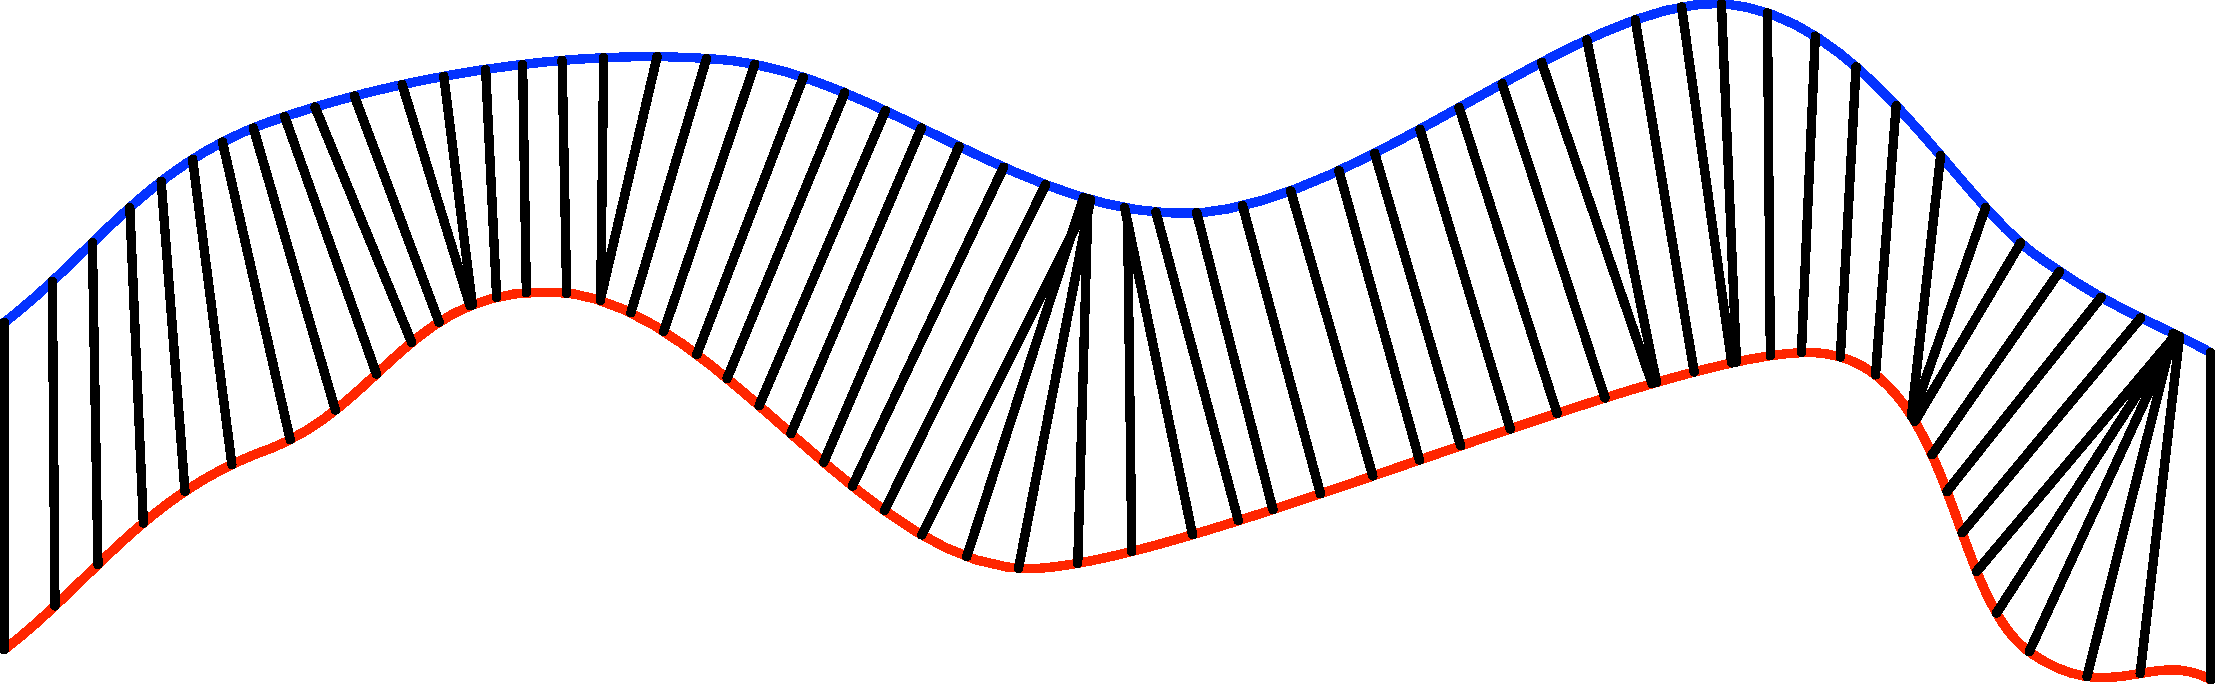
\includegraphics[width=1\textwidth]{lectSeq/dtw.pdf}

\end{frame}
%***********************************************************
\begin{frame}{Questions?}
\begin{itemize}
	\item What do we know now that we didn't know before?
\begin{itemize}
	\item We understand some of the complexities of sequential data
	\item We know some ways of making predictions for sequences
\end{itemize}

	\item How can we use what we learned today?
\begin{itemize}
	\item We can build models to classify sequences or predict from sequences
\end{itemize}
\end{itemize}
\end{frame}

\end{document}

